\documentclass[14pt, a4paper]{extarticle}

\usepackage{amsmath}

% Для XeLaTeX используем fontspec
\usepackage{fontspec}
\setmainfont{Times New Roman}  % Установим основной шрифт с поддержкой кириллицы

% Для поддержки русского языка используем polyglossia
\usepackage{polyglossia}
\setdefaultlanguage{russian}

% Указываем шрифт для кириллицы
\newfontfamily\cyrillicfont{Times New Roman}[Contextuals={WordInitial,WordFinal}]

\newfontfamily\cyrillicfonttt[Script=Cyrillic,Contextuals={WordInitial,WordFinal}]{DejaVu Sans Mono}


% Поли (ГОСТ)
\usepackage[left=3cm, right=1.5cm, top=2cm, bottom=2cm]{geometry}

% Межстрочный интервал
\usepackage{setspace}
\onehalfspacing  % 1.5 интервал

% Абзацный отступ
\setlength{\parindent}{1.25cm}

% Межабзацный интервал
\setlength{\parskip}{0pt}

% Выравнивание по ширине
\usepackage{ragged2e}
\justifying

% Заголовки разделов без автоматической нумерации и лишнего форматирования
\usepackage{titlesec}
\titleformat{\section}{\bfseries\Large}{\thesection}{1em}{}
\titleformat{\subsection}{\bfseries\large}{\thesubsection}{1em}{}
\titleformat{\subsection}[runin]{\normalfont\mdseries}{\thesubsection}{1em}{}
\titleformat{\subsection}[runin]{\normalfont\bfseries}{\thesubsection}{1em}{}

% ГОСТ библиография
\usepackage[backend=biber, style=gost-numeric, language=auto, sorting=none]{biblatex}
\addbibresource{bibliography.bib}  % Подключаем .bib файл

% Оформление рисунков и таблиц по ГОСТ
\usepackage{caption}
\captionsetup{labelsep=period,justification=centering,font=normalsize}

% Гиперссылки без цвета
\usepackage[hidelinks]{hyperref}

% Оглавление жирным
\usepackage{tocloft}
\renewcommand{\contentsname}{\bfseries Оглавление}
\renewcommand{\cftsecfont}{\bfseries}
\renewcommand{\cftsecpagefont}{\bfseries}
\renewcommand{\cfttoctitlefont}{\bfseries\Large}

\usepackage{graphicx}

\usepackage{listings}
\usepackage{xcolor} % Для настройки цветов


\usepackage{float}


\begin{document}

\begin{titlepage}
    \centering
    {\bfseries Московский государственный университет имени М.В. Ломоносова\\
    Механико-математический факультет\\
    Кафедра вычислительной математики
    }
    
    \vfill

    {\LARGE\bfseries Курсовая работа\\[1ex]
    Реализация реляционной модели логического разграничения доступа для информационных систем со сложной моделью данных}

    \vfill

    {\bfseries
    Студент: Антонов Никита Сергеевич\\[0.5ex]
    Научный руководитель: Кривчиков Максим Александрович\\[0.5ex]
    Группа: 310
    }

    \vfill

    {\bfseries Москва — 2025 г.}
\end{titlepage}

\tableofcontents
\newpage

\section*{Введение}
\addcontentsline{toc}{section}{Введение}

В условиях стремительного развития цифровых технологий и повсеместного распространения информационных систем вопросы информационной безопасности приобретают особую актуальность. Одним из ключевых направлений обеспечения защищенности данных является реализация механизмов разграничения доступа, позволяющих управлять правами пользователей в зависимости от их ролей, полномочий и контекста взаимодействия с системой.

Современные информационные системы часто оперируют сложными и взаимосвязанными наборами данных, что требует применения эффективных и масштабируемых моделей доступа. Реляционная модель логического разграничения доступа предлагает гибкий подход к контролю за доступом, основанный на использовании средств самой базы данных — в частности, через систему представлений, политик и ограничений на уровне SQL.

Цель данной курсовой работы — разработать и реализовать реляционную модель логического разграничения доступа для информационной системы, характеризующейся сложной структурой данных. В рамках исследования будет рассмотрена архитектура модели, проанализированы существующие подходы, а также предложен способ интеграции логических правил разграничения доступа в структуру реляционной базы данных.

Актуальность темы обусловлена необходимостью создания безопасных и гибко настраиваемых решений для хранения и обработки данных, соответствующих современным требованиям к защите информации. Разработка собственной модели доступа, учитывающей специфику реляционных баз данных, позволяет не только повысить уровень безопасности, но и обеспечить удобство в сопровождении и масштабировании системы.

В работе особое внимание будет уделено вопросам реализации логики разграничения на уровне SQL-запросов, использованию представлений, триггеров и других встроенных средств, обеспечивающих целостность и контролируемость доступа к данным.

%Возможно надо как-то упомянуть, что конечная цель масштабирование и интеграция в систему ИСТИНА/ЕГИСУ

\section{Результаты известных исследований}
% Текст...
Перед тем как, приступить к решению задачи, стоит изучить уже известные результаты в области исследования. Далее будут приведены несколько примеров других методов реализации разграничения доступа.
В статье \cite{Ahn1999} рассматривается модель ролевого контроля доступа Role-Based Access Control (RBAC). Основная идея - использование системы
Separation of Duty (SoD) это механизм, при котором пользователи не могут выполнять действия, которые могли бы привести к конфликту интересов(например пользователь создающий докменты, не может их утверждать)
Для этих целей был разработан язык RSL99, использующийся для описания разграничения на основе разделения обязанностей в контексте ролевого контроля доступа.
Ролевая система также описывается в статье \cite{Crampton2003}, автор делает систему более гибкой, за счет внедрения не только статических ограничений, но и динамических(ограничения зависящие, например, от времени суток, контекста, места)
Такой подхд позволяет сделать систему более детализированной и универсальной, но требует более скурпулезного подхода к безопасности, так как увеличения числа учитываемых параметров, неизбезжно повышает риск ошибки и возможности неправомерного доступа.
Рассмотрим один из базовых подходов к разграничению доступа - DAC(Discretionary Access Control). В статье \cite{Coyne1991} рассмотрен подход ACL, он довольно прост и заключается в том, что владельцы ресурсов или системные администраторы 
явно указывают, какие пользователи или группы имеют доступ к тем или иным объектам. Данный способ реализации разграничения доступа часто использууется в бизнес продуктах и системах с не очень сложной структурой данных, но для больших баз и сложных систем
он не так эффективен, этот вопрос рассматривается в статье \cite{Ellison2000}, автор указывает на возникновение человеческого фактора, а также
становится ясно, что возможность передачи правд доступа между пользователями может приводить к угрозам безопасности и в целом система DAC довльно сильно зависит от людей.
Другая более консервативная и надеждная в плане безопасности система - это MAC. Из работы \cite{FerraioloSandhu2002} можно понять главные преимущества этой системы: контроль доступа к объектам строго регулируется системой
и пользователи не могут вносить изменения в права доступа, это делает систему более защищенной от угроз и попыток неправомерного доступа, в основном MAC используется в проектах требующих серьезную безопасность данных, в ущерб гибкости.
В работе \cite{HaleNgu1994} сравниваются подходы MAC и DAC, в заключении сделан вывод, модель MAC более надежная и статичная, ее используют в системах с жесткими требованиями к безопасности,
таких как военные или политические структуры. DAC же более динамическая и гибкая структура, применяющаяся в системах не таких требовательных к безопасности, в основном базирующихся на работе с множеством людей.
Нет лучшей и универсальной модели разграничения, разработчикам важно учитывавть множество факторов системы, и исходя из этого, выбирать более подходящие пути для обеспечения безопасности данных.
Рассмотрим также более гибкие модели, близкие по свойствам к нашей конечной цели. В статье \cite{BarkaSandhu2012} рассматривается модель ABAC, в ней решения о предоставлении или отказе в  доступе основаны на атрибутах
, например, роль, возраст, местоположение и тд. За счет большого числа параметров(атрибутов) модель получается очень гибкой и хорошо подходит сложным системам с большой вариативностью данных. Но в то же время повышается и сложность сопровождения системы, проблемы с аудитом и отладкой системы.
Такие гибкие модели требуют высоких навыков от разработчиков, потому и используются не так часто, как более базовые подходы.
Другой довольно оригинальный подход к разграничению доступа - модель EBAC(Entity-Based Access Control). В работе \cite{LiYu2006} разбираются плюсы и минусы такого подхода, в отличие от модели атрибутов, модель сущностей(EBAC)
принимает решения о правах доступа на основе контекстной логики(кто создал объект, как был создан объект, в каких отношениях находятся субъекты и объекты), EBAC часто используется в системах управления знаниями и медицинских инфрмационных системах, где важны связи между пользователями, ресурсами и действиями.





\section{Постановка задачи}
% Текст...
В современных информационных системах с комплексной структурой данных важную роль играет точное и гибкое разграничение доступа.
Целью данной курсовой работы является реализация логической модели разграничения доступа на основе реляционной алгебры с последующей интеграцией в веб-приложение, разработанное на фреймворке Django.
В ходе решении задачи выполним несколько шагов:
\begin{enumerate}
    \item Определить формальные правила разграничения доступа с использованием реляционной алгебры.
    \item Спроектировать реляционную схему, отражающую эту логику.
    % \item Реализовать модель доступа в Django с учетом роли пользователя и контекста запроса.
    % \item Провести тестирование корректности работы механизма разграничения доступа.
\end{enumerate}
В результате хотим получить гибкую, корректную реляционную модель, отвечающую всем стандартным требованием к защите данных и разганичению доступа.
\section{Решение задачи}
% Текст...

\subsection{Запись правил в видел формул реляционной алгебры}
% Текст подпункта 1...
Будем по шагам выводить общую формулу запроса в терминах релляционной алгебры и в конце составим схему запроса.
Изначально объект, по которому принимается решение лежит в декартовом произведении пользователей и объектов:

\[
\text{ALL\_USERS} \times \text{ALL\_OBJECTS}
\]

Первая быстрая проверка на суперпользователя(роль, которая имеет доступ к любому объекту) :
\[
\text{is\_superuser} = \text{TRUE} \text{User} 
\]

Следующая проверка на глобальную блокировку объекта или прямой запрет пользвателю на объект :
\[
\text{NOT EXISTS}(\text{LockedObject}) \quad \text{AND} \quad \text{NOT EXISTS}(\text{DACRestriction})
\]

Здесь, LockedObject - таблица объектов, которые глобально запрещены к доступу, а DACRestriction - таблица пользователей, которым прямо запрещен доступ


Далее, если пользователь не оказался суперюзером и не имел каких-то исключений на предыдущей стадии, через цепочку проверок пользователь может получить разрешение: 

\[
\text{UserRole} \bowtie \text{Role} \bowtie \text{RolePermission}
\]

Здесь мы обращаемся к роли пользователя, каждая роль имеет RolePermission, набор разрешений, соответственно среди этих разрешений должен быть совпадающий набор действия и объекта(например чтение/редактирование, какого-то файла)

Последняя проверка, если пользователь например не имеет роли или что-то из предыдущего не было указано, в таблице DACPermission мы смотрим есть ли прямой доступ у этого пользователя к запрашиваемому объекту:
\[
\text{DACPermission}
\]


\clearpage
\subsection{Построение логической схемы и перенесение логики на код}
% Текст подпункта 2...

В этом подразделе представлена логическая схема, описанных выше правил разграничения доступа.
\begin{figure}[H]
    \centering
    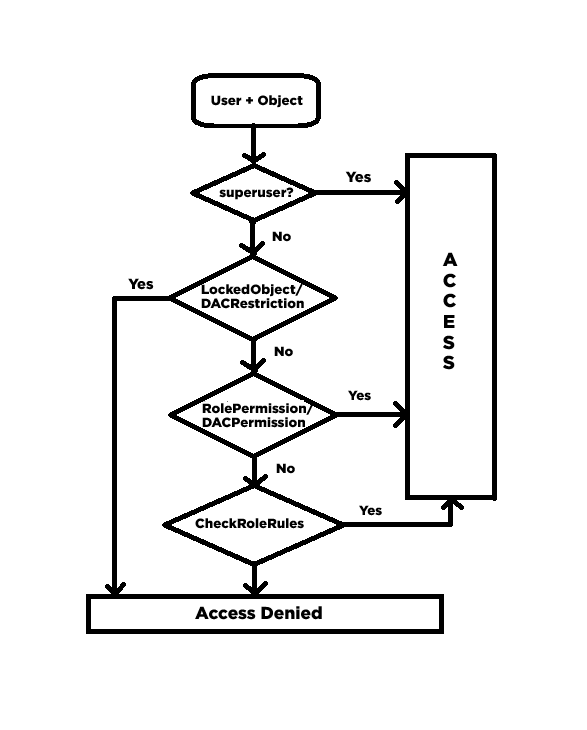
\includegraphics[width=0.8\textwidth]{SchemeLogicRed.png} % замените на имя файла
    \caption{Схема}
    \label{fig:schematic}
\end{figure}

А также программный код реализующий способ разграничения доступа к данным.

В файле models.py представлены модели данных для разграничения доступа, основные модели:
\begin{itemize}
    \item $Role$ - имя и описание роли(профессии)
    \item $RolePermission$ - для какой роли разрешение, $content_type$ - тип объекта, permission - какой тип действия разрешается
    \item $UserRole$ - связь пользователя и роли
    \item $DACPermission$ - пользователь, разрешение на конкретное действие, конкретные объект, может быть причина предоставления доступа
    \item $DACRestriction$ - аналогичное вышенаписанному, но запрет на действие
    \item $LockedObject$ - блокировка определенных прав на объект
\end{itemize}
Через эти модели реализуется управление доступом.

\lstinputlisting[language=Python, caption={Файл models.py}, label={lst:models}]{models.py}

Файл checkacces.sql реализует логику запросов, получения входных данных и предоставления прав.
По сути он описывает релляционную логику, которую мы ранее записывали формулами, а также отрисовали по ней схему.
Основные моменты это формирование по входным данным и логике, наборов правил:
\begin{itemize}
    \item $NORMAL_RULES$ - стандартные разрешения без учета блокировок
    \item $NORMAL_REPRESENTATIVE_RULES$ - разрешения, выданные через роли представителей подразделений
    \item $LOCKED_REPRESENTATIVE_RULES$ - исключения, когда роль дана через подразделение, но объект заблокирован
    \item $DAC_PERMISSION_RULES$ - индивидуальные  разрешения пользователю на объект
\end{itemize}

\lstinputlisting[language=SQL, caption={Файл checkaccess.sql}, label={lst:sql}]{checkaccess.sql}

В файле utils.py содержатся контроль над действиями над объектами, задается структура данных о доступе пользователя, также содержатся вспомогательные функции,
по типу: преобразование SQL запроса в QuerySet, получения списком объектов, а также функция компонирующая декартово произведение пользователей и объектов с разрешениями

\lstinputlisting[language=Python, caption={Файл utils.sql}, label={lst:utils}]{utils.py}





\clearpage
\section*{Заключение}
\addcontentsline{toc}{section}{Заключение}
В ходе работы мы построили логику разграничения доступа, записали ее в формулах релляционной алгебры, составили схему, иллюстрирующую логику работы модели.
Также был написан код, реализующий работу модели разграничения доступа, в фреймворке Django + SQL запросы. В дальнейшем в планах апробация и интеграция модели в систему ИСТИНА или ЕГИСУ, а также
модернизация модели под нужды соответствующей системы. На данном этапе мы получили некоторую общую логику и код релляционной модели разгарничения доступа, но ее можно будет модернизировать и улучшать, а также использовать как начальный шаблон для различных систем.
% Текст...

\newpage
\printbibliography[heading=bibintoc,title={Список литературы}]

\end{document}



